% =====================================================================
% Main-paper figures/tables reproduced FULL WIDTH (figure*/table*) in the
% two-column supplement, in v1_main order, each with a short connective note.
% The teaser is single-column so it can sit at the TOP of page 1 (a full-width
% figure* cannot: the title holds the page-1 top). The dense Limitations +
% Appendix text that follows fills the columns around the figure* floats, so
% the notes stay concise without leaving blank pages.
% Order: demo_cards -> scene_types -> factor_visual -> factor_targets ->
%        frozen_scorecard(table) -> forest -> eval_scorecard -> scale_replication
% =====================================================================

% teaser (demo_cards) moved to page 1 (after \maketitle in arxiv_combined.tex)
\section{Main-Paper Figures and Tables, Enlarged}
\label{sec:mainpaper_fullsize}

For legibility, this section reproduces each main-paper figure and the ablation table at full width, in the order they appear in the main text, with a brief note linking them.

% scene-type coverage figure moved into the MAIN body (2_data.tex) per request

\begin{figure*}[t!]
    \centering
    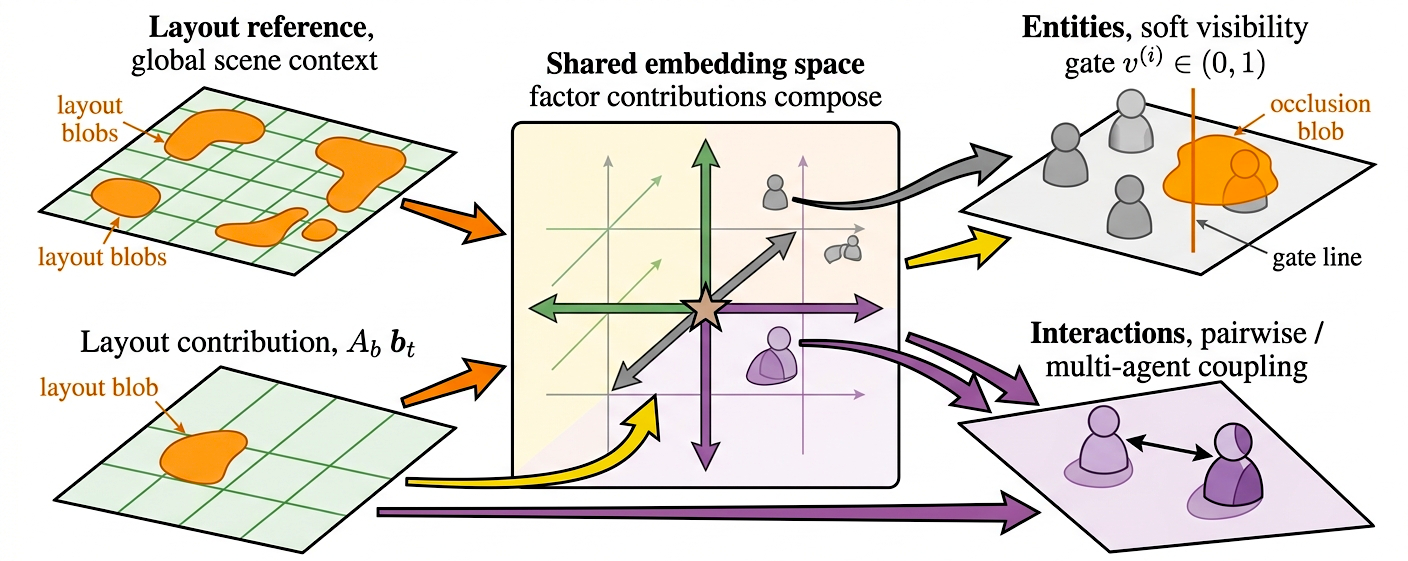
\includegraphics[width=0.88\textwidth]{figures/factor_visual.png}
    \caption{\textbf{\emph{Factorized predictive channels.}} Context is split into \emph{layout}, visibility-gated \emph{agent}, and sparse \emph{interaction} coordinates, then recomposed in the future JEPA embedding, limiting cross-factor leakage.}
    \label{fig:factorjepa_visual_full}
\end{figure*}

\noindent FactorJEPA meets this by decomposing the future into three predictive channels, layout, visibility-gated agents, and sparse interactions, recomposed in the JEPA embedding to discourage cross-factor shortcuts.

\begin{figure*}[t!]
    \centering
    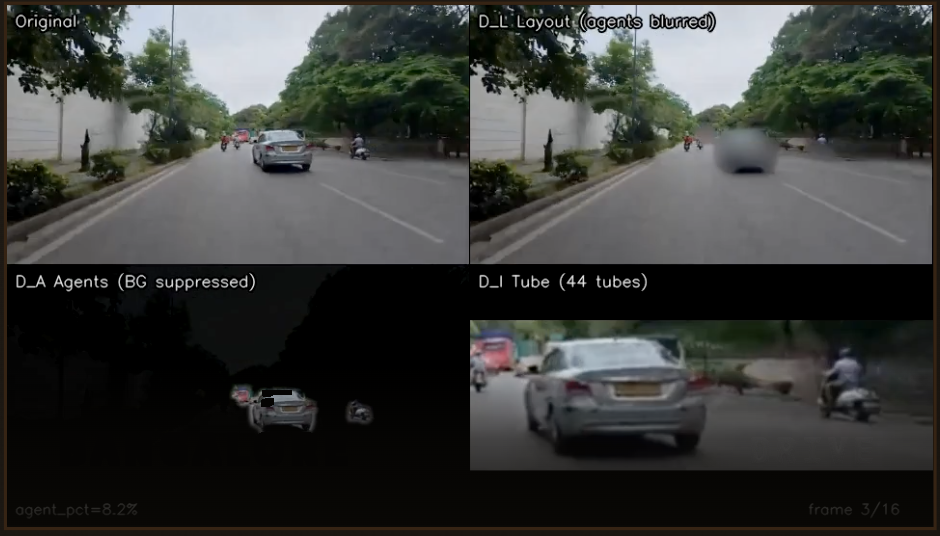
\includegraphics[width=0.88\textwidth]{figures/segmented_scene.png}
    \caption{\textbf{\emph{Automatic factor-target construction.}} Per clip, the pipeline derives \emph{layout} $D_L$, \emph{agent} $D_A$, and \emph{interaction} $D_I$ supervision by masking foreground/background and linking agent tubes.}
    \label{fig:dino_factor_targets_full}
\end{figure*}

\noindent These three views are constructed automatically by a fixed detection-and-segmentation pipeline, so the factor supervision is reproducible and scales to the full corpus without manual labels.

% frozen-encoder scorecard table moved into the MAIN body (2_factor_jepa.tex) per request

% forest / eval-scorecard / scale figures REMOVED here: they are EXACT duplicates of
% main-body Fig 7 (forest), Fig 8 (scorecard), Fig 9 (scale). factor_visual and
% segmented_scene above are kept because they are NOT in the main body.
